% \begin{frame}{Intrusion Detection}
  
%   \textbf{Intrusion Detection Systems (IDSs)}
%   \begin{itemize}
%     \item Monitor system activities (network, host, application).
%   \end{itemize}
  
% \end{frame}

\begin{frame}{Intrusion Detection}
  
  \textbf{Machine Learning (ML) for Network-based Intrusion Detection Systems (NIDSs)}
  \begin{itemize}
    \item Detect \alert{malicious} activities (\ie, \textit{misuse detection}) or \alert{anomalies} (\ie, \textit{anomaly detection}).
    \item Various types of algorithms: \alert<2>{supervised}, unsupervised, semi-supervised, reinforcement learning, \textit{etc}.
    \item Great performance with Deep Learning (DL) (on public datasets at least).
  \end{itemize}
  \bigskip
    
  \begin{figure}
    \centering
    \makebox[\textwidth][c]{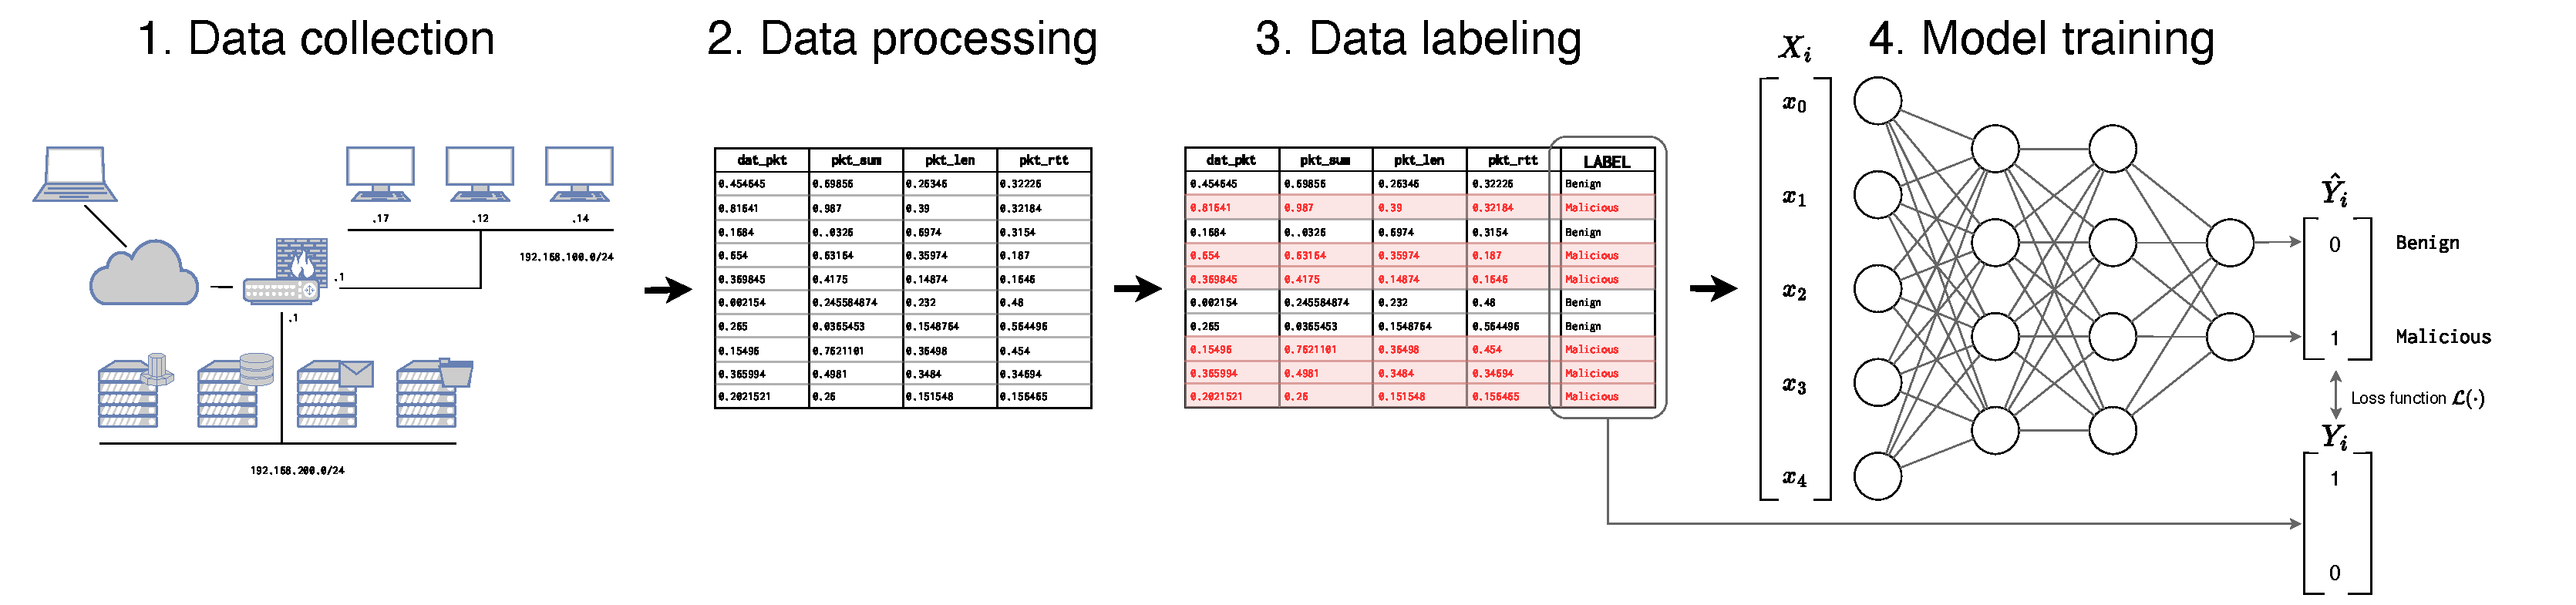
\includegraphics[width=.9\textwidth]{figures/intro/mlp-workflow.pdf}}
    \caption{Typical workflow for ML-based NIDSs.}
  \end{figure}
\end{frame}

\begin{frame}{Intrusion Detection}

  \begin{columns}
    \begin{column}{0.5\textwidth}
        \textbf{Challenges:}
        \begin{itemize}
          \item not enough labelled data;
          \item risk of local bias or skewed data distribution;
          \item inefficient against new attacks, especially \alert{supervised} approaches.
        \end{itemize}
    \end{column}

    \begin{column}{0.5\textwidth}
      \begin{figure}
        \centering
        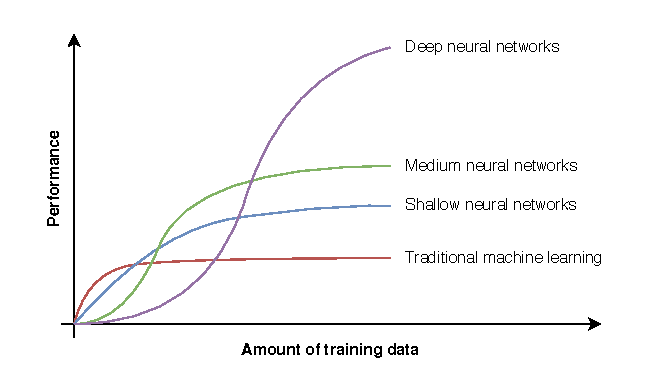
\includegraphics[width=\linewidth]{figures/intro/ml-perf}
      \end{figure}
    \end{column}
  \end{columns}
\end{frame}

\begin{frame}{Scaling Intrusion Detection}

  \textbf{Federated Learning (FL)}
  
  \begin{itemize}
    \item Novel-\emph{ish} distributed ML paradigm (Google, 2017)~\cite{mcmahan_Communicationefficientlearningdeep_2017}.
    \item Distributed clients can train a common model without sharing their training data.
    \item Privacy-preserving: high level of abstraction for the shared models preventing data leakage.
  \end{itemize}
\end{frame}

\begin{frame}{FL Fundamentals}
  \vspace{-1em}
  \begin{figure}
    \centering
    \only<1>{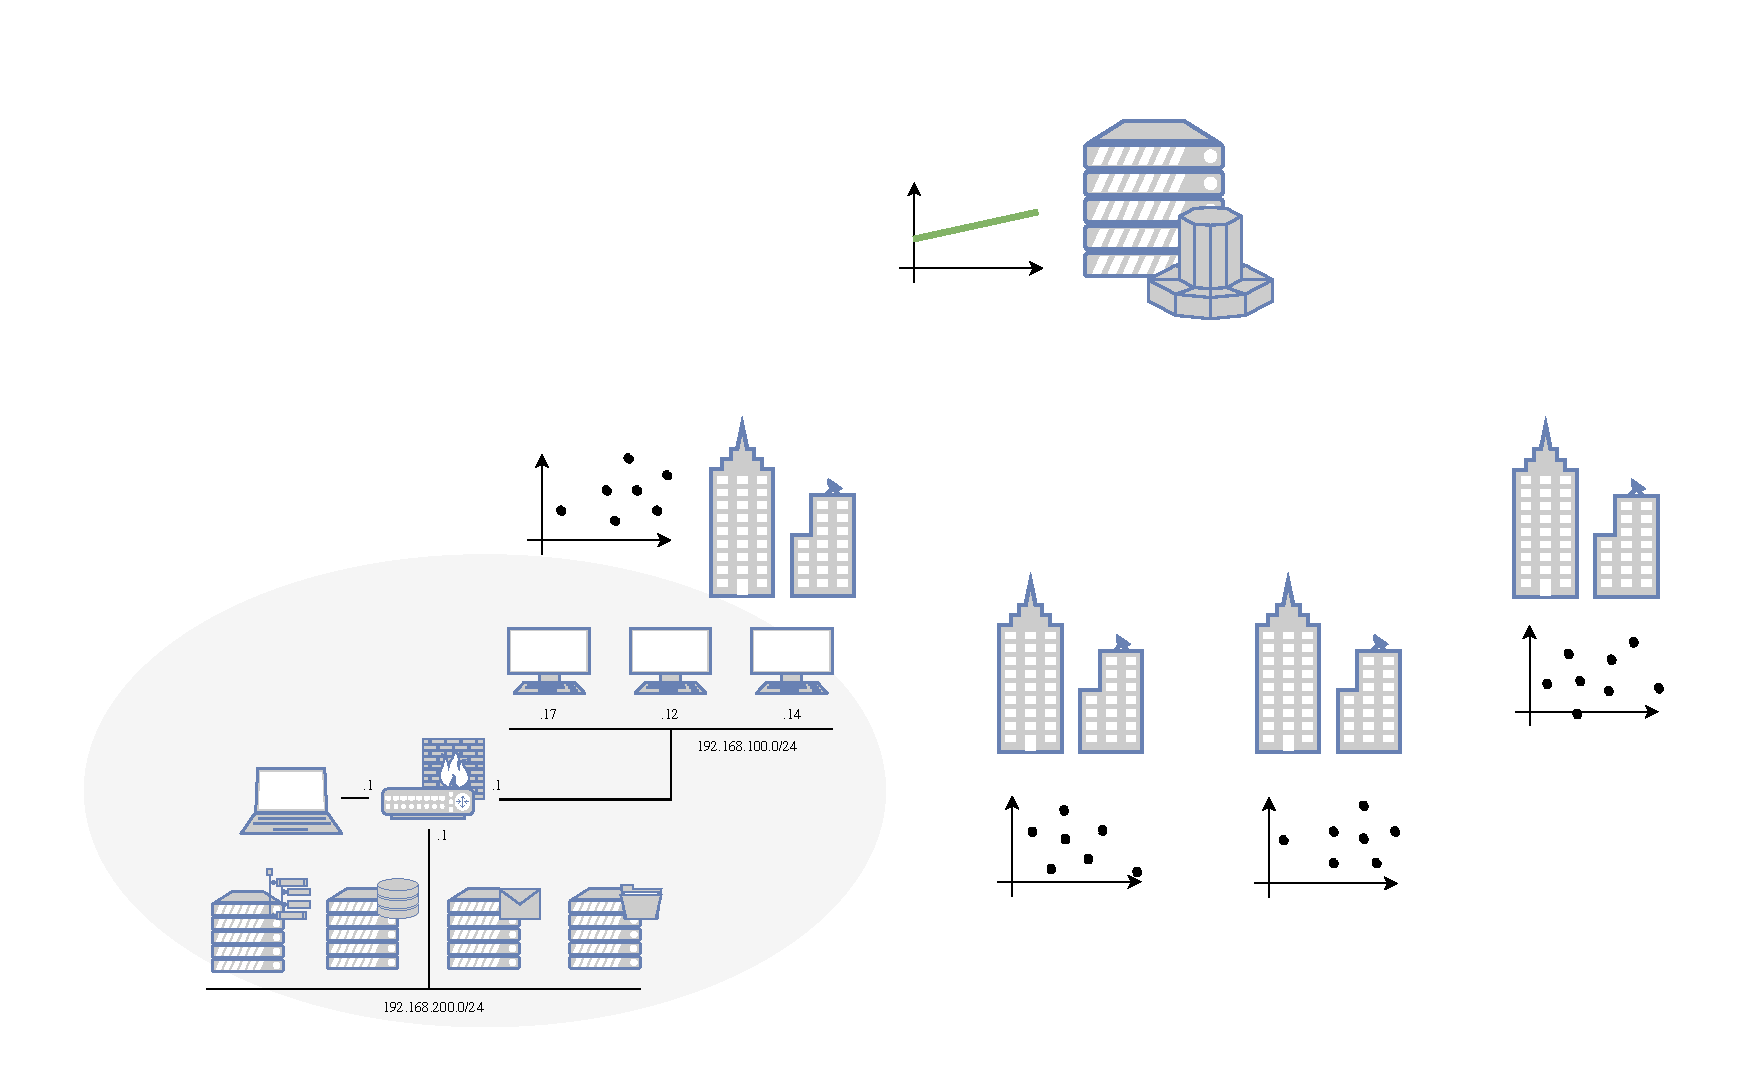
\includegraphics[width=.75\linewidth]{./figures/intro/fl/0.pdf}}%
    \only<2>{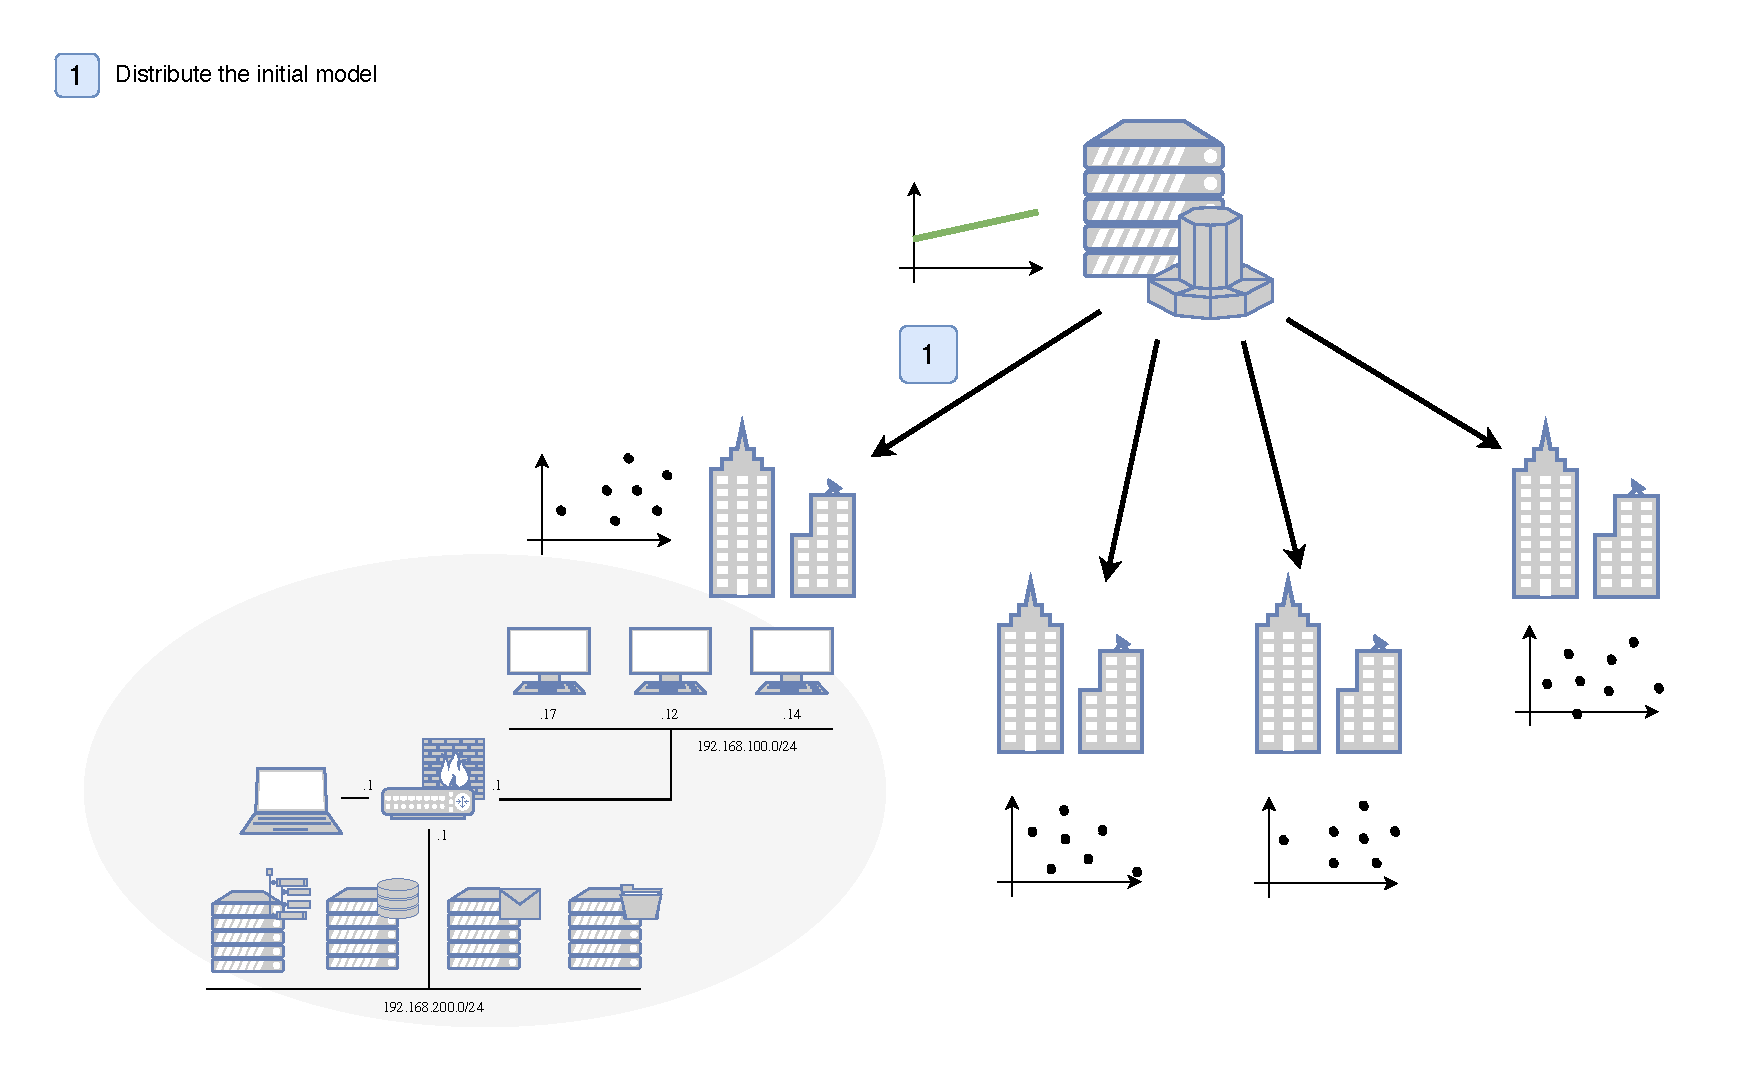
\includegraphics[width=.75\linewidth]{./figures/intro/fl/1.pdf}}%
    % Cannot use animations with MacOS Preview.
    % \only<3>{\animategraphics[width=.75\linewidth,loop,autoplay]{2}{./figures/intro/fl/2-}{1}{2}}%
    \only<3>{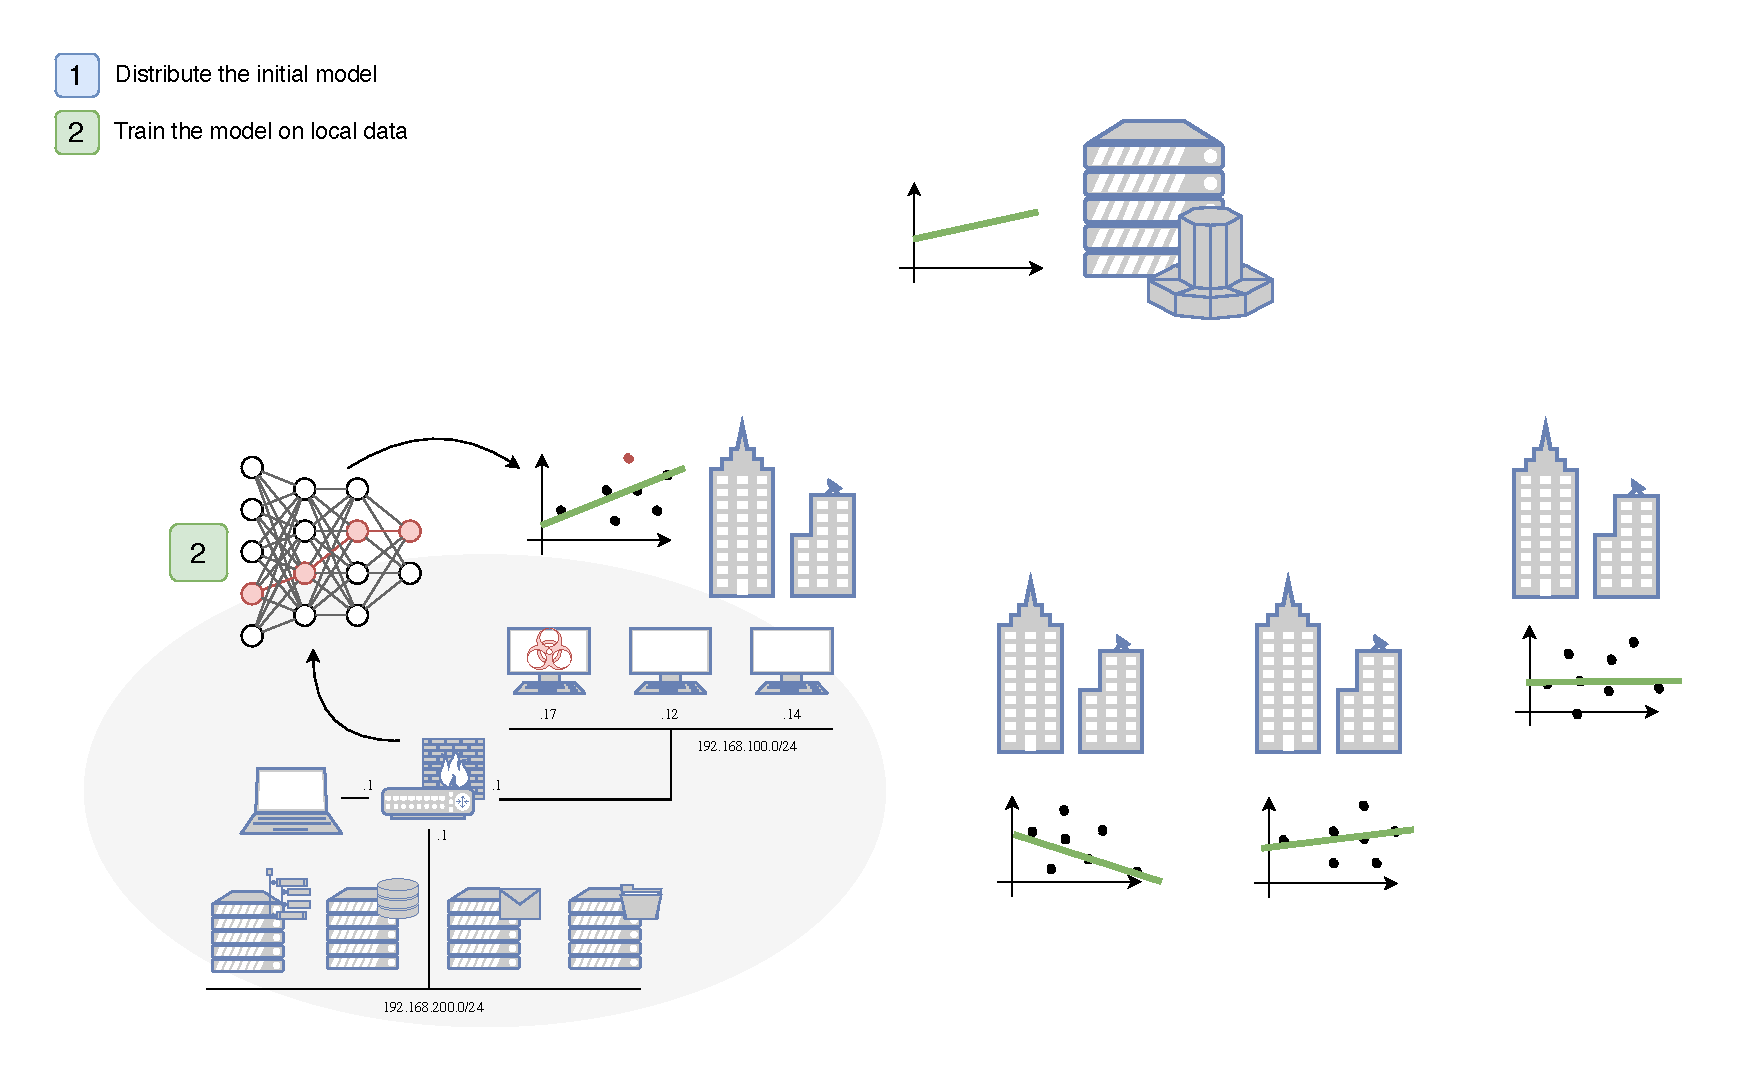
\includegraphics[width=.75\linewidth]{./figures/intro/fl/2-2.pdf}}%
    \only<4>{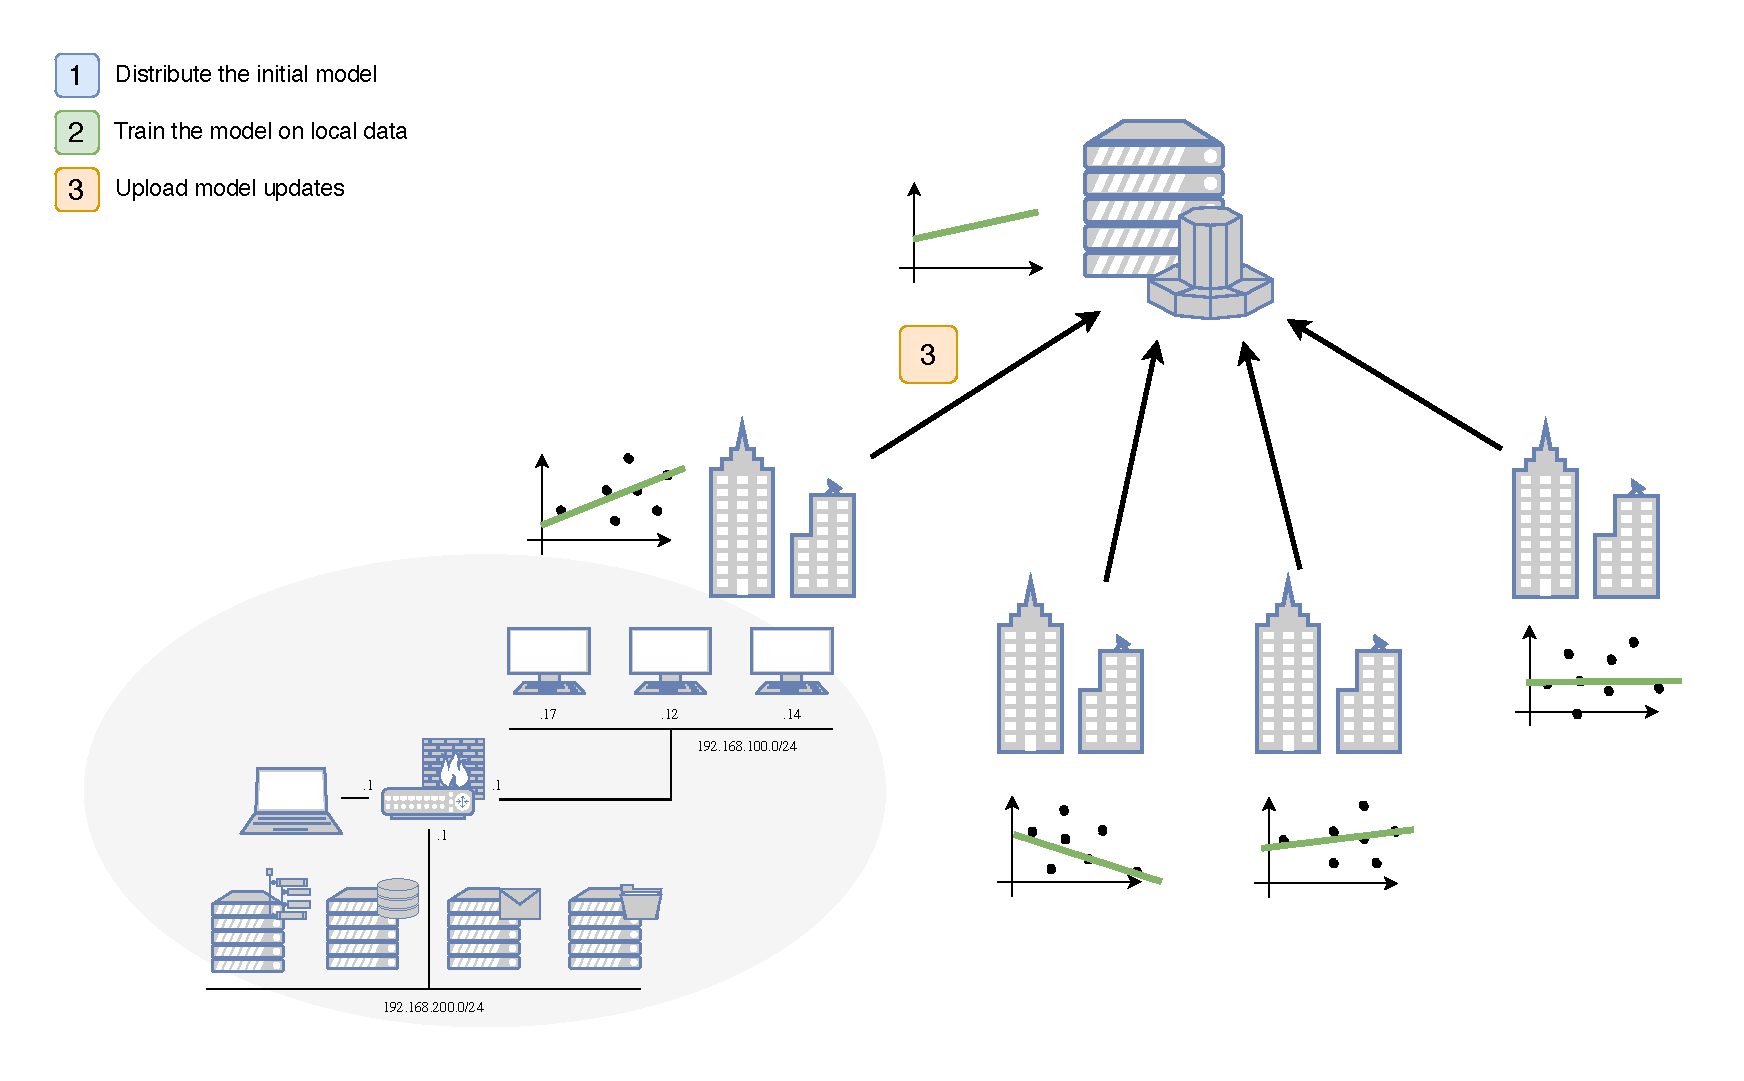
\includegraphics[width=.75\linewidth]{./figures/intro/fl/3.pdf}}%
    \only<5>{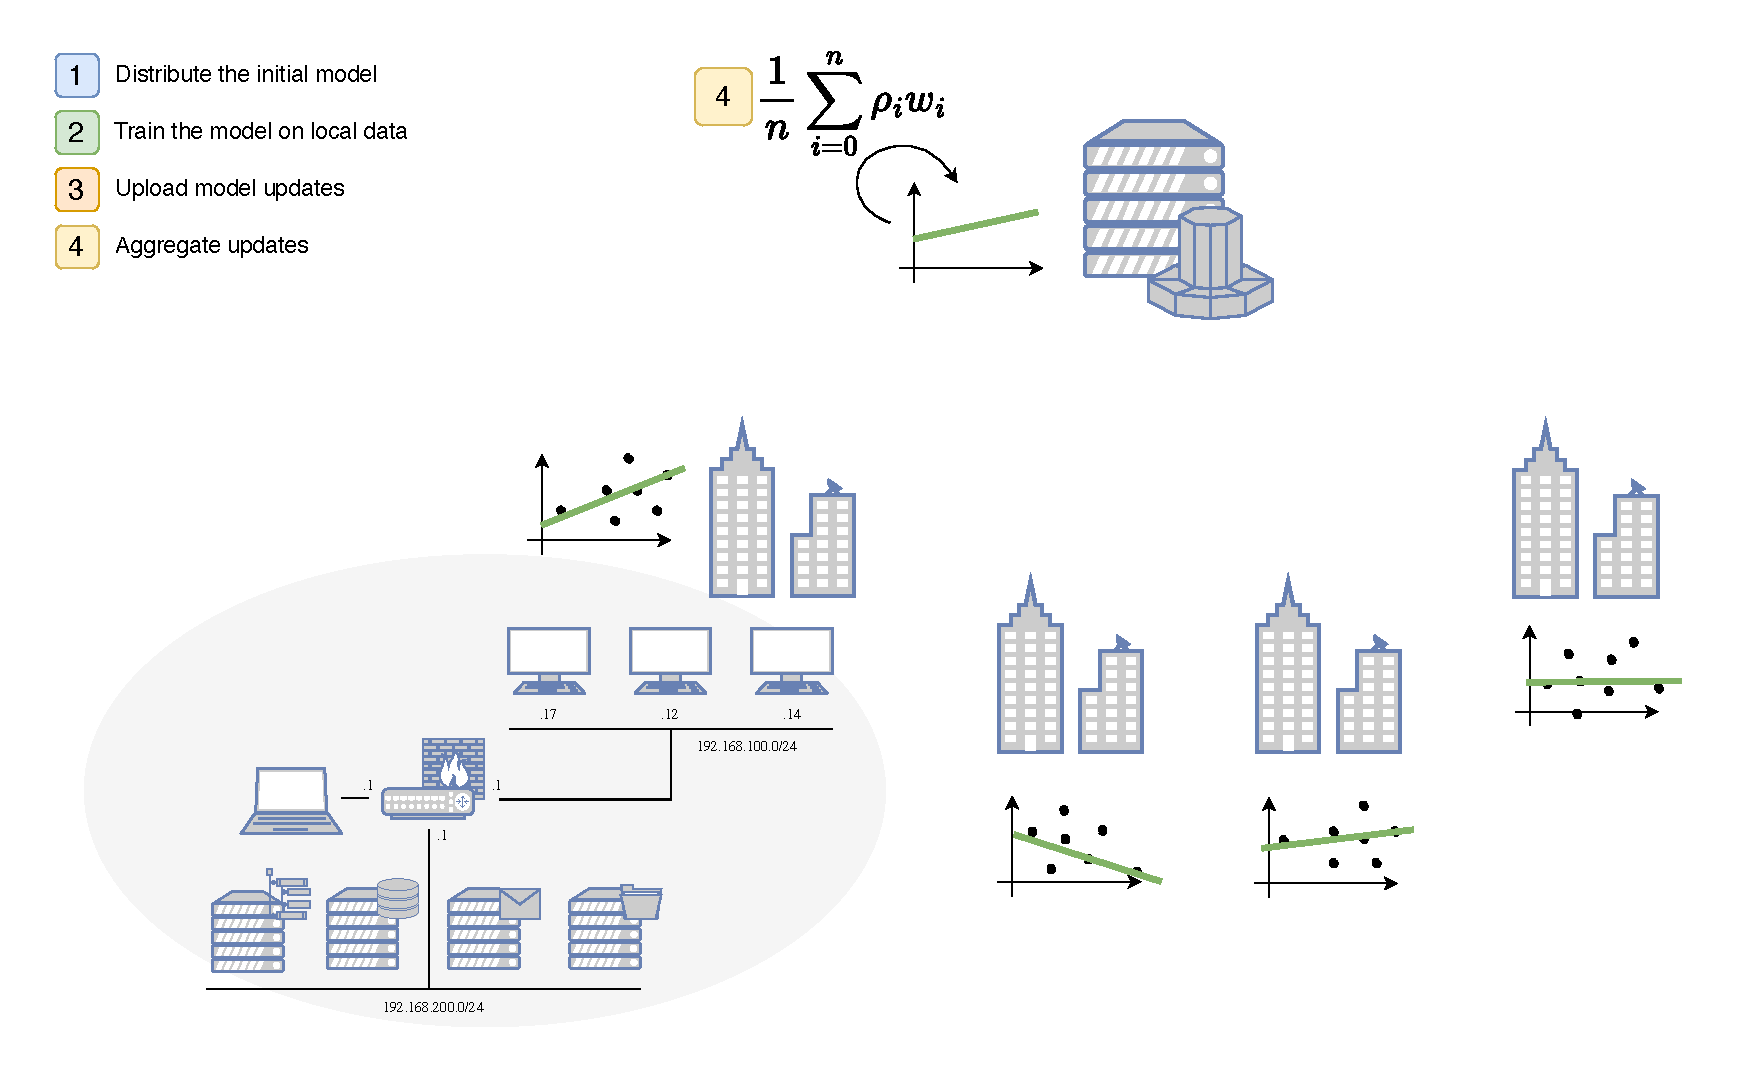
\includegraphics[width=.75\linewidth]{./figures/intro/fl/4.pdf}}%
    \only<6>{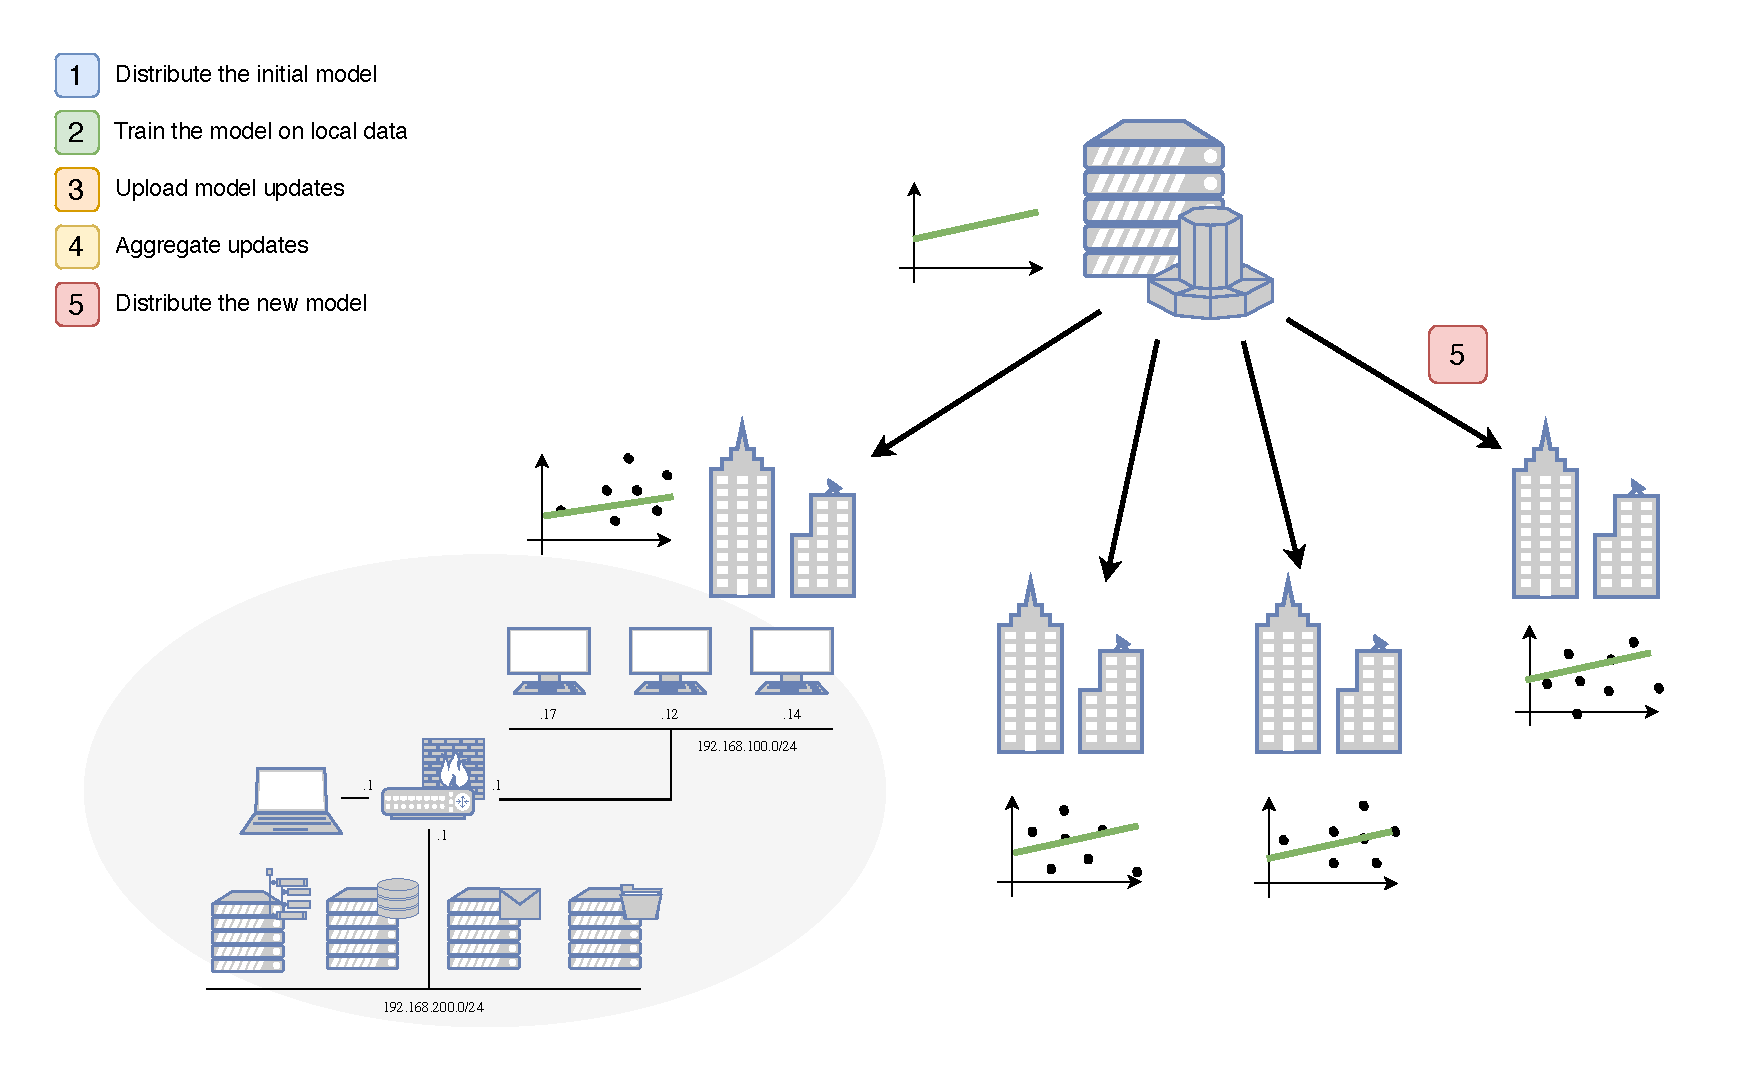
\includegraphics[width=.75\linewidth]{./figures/intro/fl/5.pdf}}%
    \only<7>{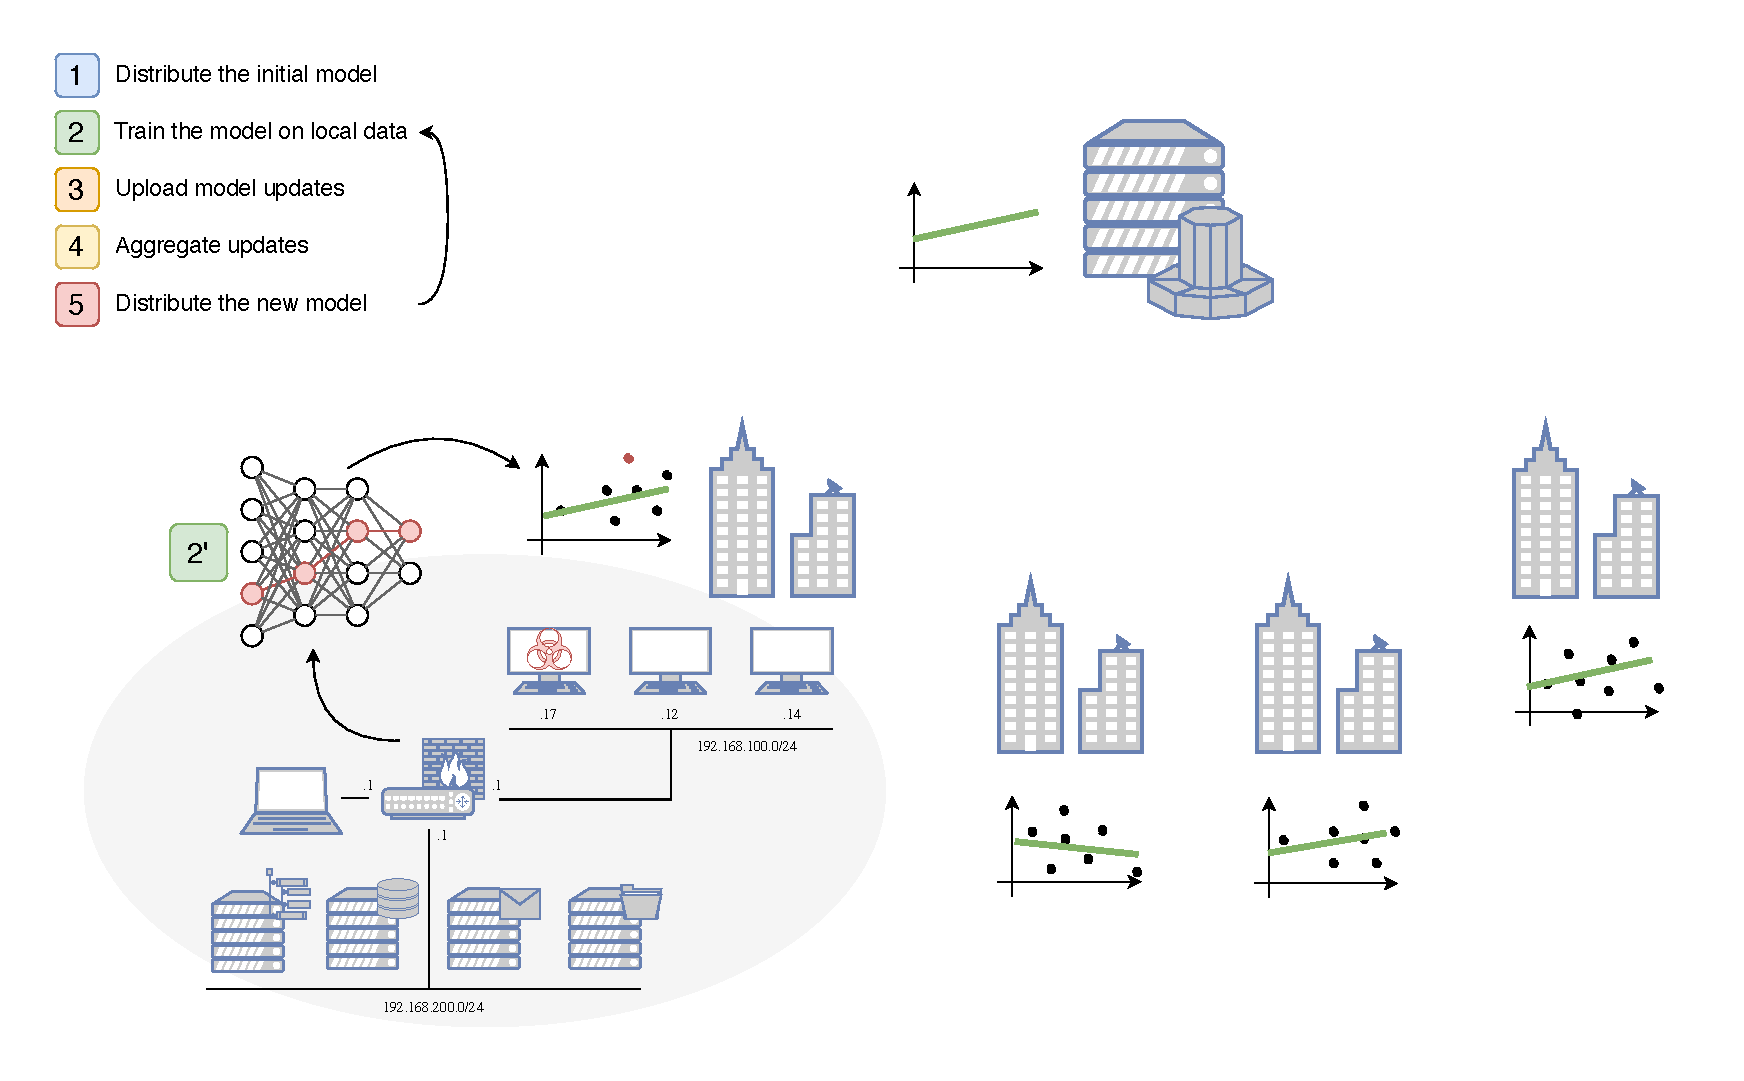
\includegraphics[width=.75\linewidth]{./figures/intro/fl/6.pdf}}%
    \caption{Typical FL workflow, applied to NIDSs.}
  \end{figure}
\end{frame}

\begin{frame}{FL for NIDSs}

  \textbf{Benefits}
  \begin{itemize}[<+->]
    \item Virtually extended dataset with Horizontal FL.
    \begin{itemize}[<1->]
      \item Better generalization.
      \item Reduced risk of overfitting or local bias.
    \end{itemize}
    

    \item Effectively share knowledge (\eg, on specific classes, instances) between participants
    \begin{itemize}[<1->]
      \item Share the knowledge about a new attack~\autocite{lavaur_icdcs_demo_2024};
      \item Improve the characterization of specific devices; \dots
    \end{itemize}

    \only<2>{\fcitefootnote{lavaur_icdcs_demo_2024}}

  \end{itemize}
\end{frame}

\begin{frame}{Case Study}
  \textbf{Collaborative Intrusion Detection between Distributed Organizations}
  \begin{itemize}
    \item Each organization has its own NIDS and monitors an information system.
    \item They want to improve their detection capabilities.
    \item Share knowledge about new attacks or specific devices.
  \end{itemize}

  \onslide<2->{%
    \textbf{A cross-silo use case:}
    \begin{itemize}
      \item few clients (\ie, 10——100);
      \item consequent amount of data, high heterogeneity;
      \item high availability, significant computing resources.
    \end{itemize}
  }
\end{frame}

\begin{frame}{Heterogeneity Headaches}
  
  \begin{columns}
    \begin{column}{.5\textwidth}
      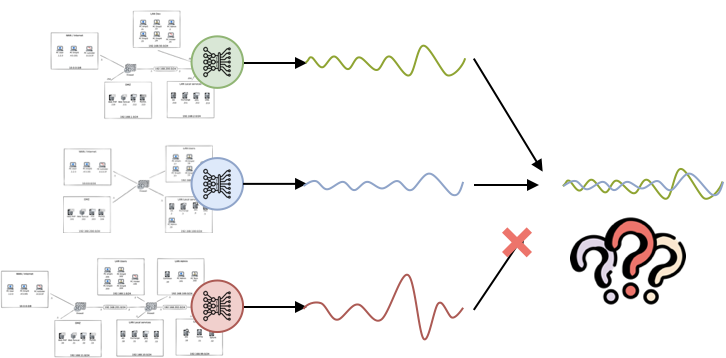
\includegraphics[width=\linewidth]{figures/intro/heterogeneity.png}
    \end{column}

    \begin{column}{.5\textwidth}

      \textcolor<2->{lightgray}{%
      \textbf{Challenge I}: \textit{Too much heterogeneity leads to poor performance\dots}
      }
      \only<1>{%
        \begin{itemize} \small
          \item How to handle different feature sets, data distributions?
          \item How to consider models that are dissimilar because they "contain" relevant knowledge?
        \end{itemize}
      }
      \vspace{1ex}


      \textcolor<1,3>{lightgray}{%
      \textbf{Challenge II}: \textit{Difficult to identify malicious contributions when models are different\dots}
      }
      
      \only<2>{%
        \begin{itemize} \small
          \item Are model "dissimilar" because they are different, or because they are malicious/poisoned?
        \end{itemize}
      }
      \vspace{1ex}
      
      \only<1-2>{\color{lightgray}}
      \textbf{Challenge III}: \textit{No representative dataset of heterogeneous distributed intrusion detection\dots}~\only<3>{\autocite{lavaur_cesar_2022}}
      
      \only<3>{%
      \begin{itemize} \small
          \item Datasets are generated locally, lots of different feature sets, no control over heterogeneity.
        \end{itemize}
      }%
    \end{column}
  \end{columns}

  \only<3>{\fcitefootnote{lavaur_cesar_2022}}
  
\end{frame}

\begin{frame}{Research Questions}
  \begin{enumerate}
    \item What makes applying FL to IDSs specific?
    \item Can FL be used to federate IDSs across heterogeneous data sources?
    \item How does FL handle malicious contributions in a federated IDS?
    \item How can one assess and ensure the trustworthiness of the other participants’ contributions?
  \end{enumerate}
\end{frame}